% Created by tikzDevice version 0.12.3 on 2019-09-27 15:30:23
% !TEX encoding = UTF-8 Unicode
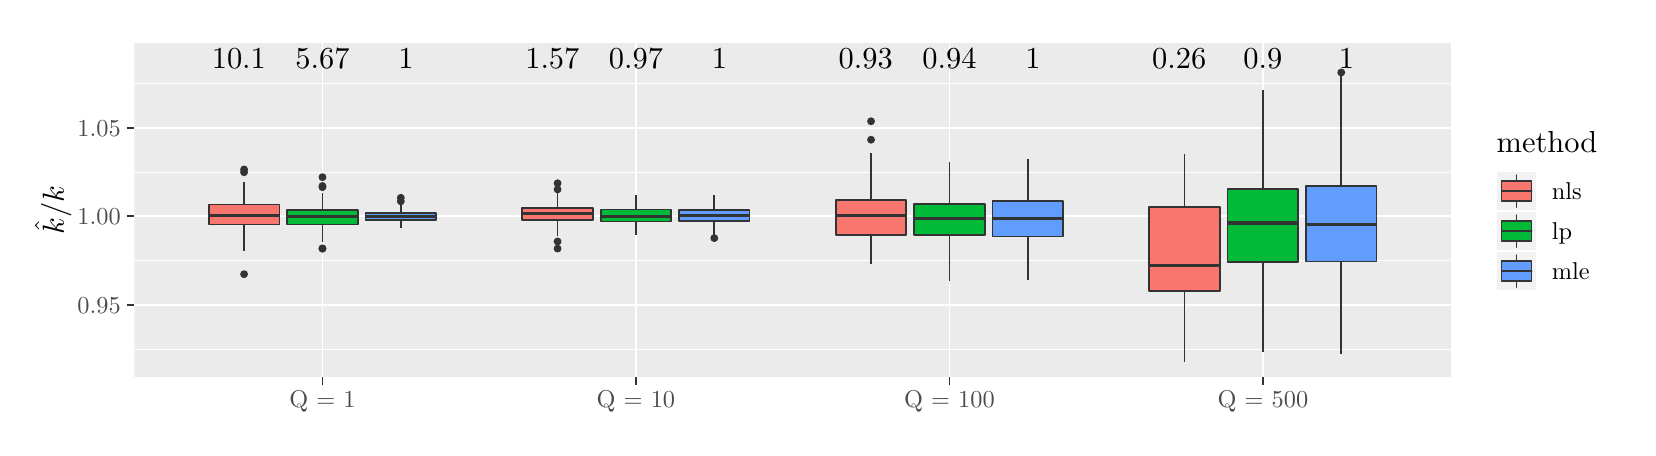
\begin{tikzpicture}[x=1pt,y=1pt]
\definecolor{fillColor}{RGB}{255,255,255}
\path[use as bounding box,fill=fillColor,fill opacity=0.00] (0,0) rectangle (578.16,144.54);
\begin{scope}
\path[clip] (  0.00,  0.00) rectangle (578.16,144.54);
\definecolor{drawColor}{RGB}{255,255,255}
\definecolor{fillColor}{RGB}{255,255,255}

\path[draw=drawColor,line width= 0.6pt,line join=round,line cap=round,fill=fillColor] (  0.00,  0.00) rectangle (578.16,144.54);
\end{scope}
\begin{scope}
\path[clip] ( 38.56, 18.22) rectangle (514.31,139.04);
\definecolor{fillColor}{gray}{0.92}

\path[fill=fillColor] ( 38.56, 18.22) rectangle (514.31,139.04);
\definecolor{drawColor}{RGB}{255,255,255}

\path[draw=drawColor,line width= 0.3pt,line join=round] ( 38.56, 28.41) --
	(514.31, 28.41);

\path[draw=drawColor,line width= 0.3pt,line join=round] ( 38.56, 60.40) --
	(514.31, 60.40);

\path[draw=drawColor,line width= 0.3pt,line join=round] ( 38.56, 92.40) --
	(514.31, 92.40);

\path[draw=drawColor,line width= 0.3pt,line join=round] ( 38.56,124.40) --
	(514.31,124.40);

\path[draw=drawColor,line width= 0.6pt,line join=round] ( 38.56, 44.40) --
	(514.31, 44.40);

\path[draw=drawColor,line width= 0.6pt,line join=round] ( 38.56, 76.40) --
	(514.31, 76.40);

\path[draw=drawColor,line width= 0.6pt,line join=round] ( 38.56,108.40) --
	(514.31,108.40);

\path[draw=drawColor,line width= 0.6pt,line join=round] (106.52, 18.22) --
	(106.52,139.04);

\path[draw=drawColor,line width= 0.6pt,line join=round] (219.79, 18.22) --
	(219.79,139.04);

\path[draw=drawColor,line width= 0.6pt,line join=round] (333.07, 18.22) --
	(333.07,139.04);

\path[draw=drawColor,line width= 0.6pt,line join=round] (446.34, 18.22) --
	(446.34,139.04);
\definecolor{drawColor}{gray}{0.20}
\definecolor{fillColor}{gray}{0.20}

\path[draw=drawColor,line width= 0.4pt,line join=round,line cap=round,fill=fillColor] ( 78.20, 55.46) circle (  1.21);

\path[draw=drawColor,line width= 0.4pt,line join=round,line cap=round,fill=fillColor] ( 78.20, 92.30) circle (  1.21);

\path[draw=drawColor,line width= 0.4pt,line join=round,line cap=round,fill=fillColor] ( 78.20, 93.32) circle (  1.21);

\path[draw=drawColor,line width= 0.6pt,line join=round] ( 78.20, 80.59) -- ( 78.20, 88.87);

\path[draw=drawColor,line width= 0.6pt,line join=round] ( 78.20, 73.42) -- ( 78.20, 63.72);
\definecolor{fillColor}{RGB}{248,118,109}

\path[draw=drawColor,line width= 0.6pt,line join=round,line cap=round,fill=fillColor] ( 65.46, 80.59) --
	( 65.46, 73.42) --
	( 90.94, 73.42) --
	( 90.94, 80.59) --
	( 65.46, 80.59) --
	cycle;

\path[draw=drawColor,line width= 1.1pt,line join=round] ( 65.46, 76.59) -- ( 90.94, 76.59);
\definecolor{fillColor}{gray}{0.20}

\path[draw=drawColor,line width= 0.4pt,line join=round,line cap=round,fill=fillColor] (106.52, 87.34) circle (  1.21);

\path[draw=drawColor,line width= 0.4pt,line join=round,line cap=round,fill=fillColor] (106.52, 86.90) circle (  1.21);

\path[draw=drawColor,line width= 0.4pt,line join=round,line cap=round,fill=fillColor] (106.52, 64.78) circle (  1.21);

\path[draw=drawColor,line width= 0.4pt,line join=round,line cap=round,fill=fillColor] (106.52, 64.68) circle (  1.21);

\path[draw=drawColor,line width= 0.4pt,line join=round,line cap=round,fill=fillColor] (106.52, 90.52) circle (  1.21);

\path[draw=drawColor,line width= 0.6pt,line join=round] (106.52, 78.57) -- (106.52, 84.84);

\path[draw=drawColor,line width= 0.6pt,line join=round] (106.52, 73.40) -- (106.52, 67.20);
\definecolor{fillColor}{RGB}{0,186,56}

\path[draw=drawColor,line width= 0.6pt,line join=round,line cap=round,fill=fillColor] ( 93.78, 78.57) --
	( 93.78, 73.40) --
	(119.26, 73.40) --
	(119.26, 78.57) --
	( 93.78, 78.57) --
	cycle;

\path[draw=drawColor,line width= 1.1pt,line join=round] ( 93.78, 76.15) -- (119.26, 76.15);
\definecolor{fillColor}{gray}{0.20}

\path[draw=drawColor,line width= 0.4pt,line join=round,line cap=round,fill=fillColor] (134.84, 81.80) circle (  1.21);

\path[draw=drawColor,line width= 0.4pt,line join=round,line cap=round,fill=fillColor] (134.84, 83.06) circle (  1.21);

\path[draw=drawColor,line width= 0.6pt,line join=round] (134.84, 77.48) -- (134.84, 80.80);

\path[draw=drawColor,line width= 0.6pt,line join=round] (134.84, 75.07) -- (134.84, 72.01);
\definecolor{fillColor}{RGB}{97,156,255}

\path[draw=drawColor,line width= 0.6pt,line join=round,line cap=round,fill=fillColor] (122.09, 77.48) --
	(122.09, 75.07) --
	(147.58, 75.07) --
	(147.58, 77.48) --
	(122.09, 77.48) --
	cycle;

\path[draw=drawColor,line width= 1.1pt,line join=round] (122.09, 76.33) -- (147.58, 76.33);
\definecolor{fillColor}{gray}{0.20}

\path[draw=drawColor,line width= 0.4pt,line join=round,line cap=round,fill=fillColor] (191.48, 67.28) circle (  1.21);

\path[draw=drawColor,line width= 0.4pt,line join=round,line cap=round,fill=fillColor] (191.48, 86.10) circle (  1.21);

\path[draw=drawColor,line width= 0.4pt,line join=round,line cap=round,fill=fillColor] (191.48, 88.32) circle (  1.21);

\path[draw=drawColor,line width= 0.4pt,line join=round,line cap=round,fill=fillColor] (191.48, 64.72) circle (  1.21);

\path[draw=drawColor,line width= 0.6pt,line join=round] (191.48, 79.34) -- (191.48, 85.03);

\path[draw=drawColor,line width= 0.6pt,line join=round] (191.48, 74.95) -- (191.48, 69.30);
\definecolor{fillColor}{RGB}{248,118,109}

\path[draw=drawColor,line width= 0.6pt,line join=round,line cap=round,fill=fillColor] (178.73, 79.34) --
	(178.73, 74.95) --
	(204.22, 74.95) --
	(204.22, 79.34) --
	(178.73, 79.34) --
	cycle;

\path[draw=drawColor,line width= 1.1pt,line join=round] (178.73, 77.45) -- (204.22, 77.45);

\path[draw=drawColor,line width= 0.6pt,line join=round] (219.79, 78.81) -- (219.79, 84.01);

\path[draw=drawColor,line width= 0.6pt,line join=round] (219.79, 74.53) -- (219.79, 69.58);
\definecolor{fillColor}{RGB}{0,186,56}

\path[draw=drawColor,line width= 0.6pt,line join=round,line cap=round,fill=fillColor] (207.05, 78.81) --
	(207.05, 74.53) --
	(232.54, 74.53) --
	(232.54, 78.81) --
	(207.05, 78.81) --
	cycle;

\path[draw=drawColor,line width= 1.1pt,line join=round] (207.05, 76.43) -- (232.54, 76.43);
\definecolor{fillColor}{gray}{0.20}

\path[draw=drawColor,line width= 0.4pt,line join=round,line cap=round,fill=fillColor] (248.11, 68.50) circle (  1.21);

\path[draw=drawColor,line width= 0.6pt,line join=round] (248.11, 78.57) -- (248.11, 84.08);

\path[draw=drawColor,line width= 0.6pt,line join=round] (248.11, 74.61) -- (248.11, 69.16);
\definecolor{fillColor}{RGB}{97,156,255}

\path[draw=drawColor,line width= 0.6pt,line join=round,line cap=round,fill=fillColor] (235.37, 78.57) --
	(235.37, 74.61) --
	(260.86, 74.61) --
	(260.86, 78.57) --
	(235.37, 78.57) --
	cycle;

\path[draw=drawColor,line width= 1.1pt,line join=round] (235.37, 76.61) -- (260.86, 76.61);
\definecolor{fillColor}{gray}{0.20}

\path[draw=drawColor,line width= 0.4pt,line join=round,line cap=round,fill=fillColor] (304.75,104.05) circle (  1.21);

\path[draw=drawColor,line width= 0.4pt,line join=round,line cap=round,fill=fillColor] (304.75,110.72) circle (  1.21);

\path[draw=drawColor,line width= 0.6pt,line join=round] (304.75, 82.36) -- (304.75, 99.20);

\path[draw=drawColor,line width= 0.6pt,line join=round] (304.75, 69.66) -- (304.75, 59.21);
\definecolor{fillColor}{RGB}{248,118,109}

\path[draw=drawColor,line width= 0.6pt,line join=round,line cap=round,fill=fillColor] (292.01, 82.36) --
	(292.01, 69.66) --
	(317.49, 69.66) --
	(317.49, 82.36) --
	(292.01, 82.36) --
	cycle;

\path[draw=drawColor,line width= 1.1pt,line join=round] (292.01, 76.76) -- (317.49, 76.76);

\path[draw=drawColor,line width= 0.6pt,line join=round] (333.07, 80.87) -- (333.07, 96.15);

\path[draw=drawColor,line width= 0.6pt,line join=round] (333.07, 69.69) -- (333.07, 52.93);
\definecolor{fillColor}{RGB}{0,186,56}

\path[draw=drawColor,line width= 0.6pt,line join=round,line cap=round,fill=fillColor] (320.33, 80.87) --
	(320.33, 69.69) --
	(345.81, 69.69) --
	(345.81, 80.87) --
	(320.33, 80.87) --
	cycle;

\path[draw=drawColor,line width= 1.1pt,line join=round] (320.33, 75.73) -- (345.81, 75.73);

\path[draw=drawColor,line width= 0.6pt,line join=round] (361.39, 81.90) -- (361.39, 96.93);

\path[draw=drawColor,line width= 0.6pt,line join=round] (361.39, 69.14) -- (361.39, 53.31);
\definecolor{fillColor}{RGB}{97,156,255}

\path[draw=drawColor,line width= 0.6pt,line join=round,line cap=round,fill=fillColor] (348.64, 81.90) --
	(348.64, 69.14) --
	(374.13, 69.14) --
	(374.13, 81.90) --
	(348.64, 81.90) --
	cycle;

\path[draw=drawColor,line width= 1.1pt,line join=round] (348.64, 75.50) -- (374.13, 75.50);

\path[draw=drawColor,line width= 0.6pt,line join=round] (418.02, 79.67) -- (418.02, 98.88);

\path[draw=drawColor,line width= 0.6pt,line join=round] (418.02, 49.38) -- (418.02, 23.71);
\definecolor{fillColor}{RGB}{248,118,109}

\path[draw=drawColor,line width= 0.6pt,line join=round,line cap=round,fill=fillColor] (405.28, 79.67) --
	(405.28, 49.38) --
	(430.77, 49.38) --
	(430.77, 79.67) --
	(405.28, 79.67) --
	cycle;

\path[draw=drawColor,line width= 1.1pt,line join=round] (405.28, 58.61) -- (430.77, 58.61);

\path[draw=drawColor,line width= 0.6pt,line join=round] (446.34, 86.16) -- (446.34,122.00);

\path[draw=drawColor,line width= 0.6pt,line join=round] (446.34, 59.95) -- (446.34, 27.19);
\definecolor{fillColor}{RGB}{0,186,56}

\path[draw=drawColor,line width= 0.6pt,line join=round,line cap=round,fill=fillColor] (433.60, 86.16) --
	(433.60, 59.95) --
	(459.09, 59.95) --
	(459.09, 86.16) --
	(433.60, 86.16) --
	cycle;

\path[draw=drawColor,line width= 1.1pt,line join=round] (433.60, 73.95) -- (459.09, 73.95);
\definecolor{fillColor}{gray}{0.20}

\path[draw=drawColor,line width= 0.4pt,line join=round,line cap=round,fill=fillColor] (474.66,128.35) circle (  1.21);

\path[draw=drawColor,line width= 0.6pt,line join=round] (474.66, 87.27) -- (474.66,127.01);

\path[draw=drawColor,line width= 0.6pt,line join=round] (474.66, 60.08) -- (474.66, 26.46);
\definecolor{fillColor}{RGB}{97,156,255}

\path[draw=drawColor,line width= 0.6pt,line join=round,line cap=round,fill=fillColor] (461.92, 87.27) --
	(461.92, 60.08) --
	(487.40, 60.08) --
	(487.40, 87.27) --
	(461.92, 87.27) --
	cycle;

\path[draw=drawColor,line width= 1.1pt,line join=round] (461.92, 73.58) -- (487.40, 73.58);
\definecolor{drawColor}{RGB}{0,0,0}

\node[text=drawColor,anchor=base,inner sep=0pt, outer sep=0pt, scale=  1.10] at (136.73,129.75) {1};

\node[text=drawColor,anchor=base,inner sep=0pt, outer sep=0pt, scale=  1.10] at (106.52,129.75) {5.67};

\node[text=drawColor,anchor=base,inner sep=0pt, outer sep=0pt, scale=  1.10] at ( 76.31,129.75) {10.1};

\node[text=drawColor,anchor=base,inner sep=0pt, outer sep=0pt, scale=  1.10] at (250.00,129.75) {1};

\node[text=drawColor,anchor=base,inner sep=0pt, outer sep=0pt, scale=  1.10] at (219.79,129.75) {0.97};

\node[text=drawColor,anchor=base,inner sep=0pt, outer sep=0pt, scale=  1.10] at (189.59,129.75) {1.57};

\node[text=drawColor,anchor=base,inner sep=0pt, outer sep=0pt, scale=  1.10] at (363.28,129.75) {1};

\node[text=drawColor,anchor=base,inner sep=0pt, outer sep=0pt, scale=  1.10] at (333.07,129.75) {0.94};

\node[text=drawColor,anchor=base,inner sep=0pt, outer sep=0pt, scale=  1.10] at (302.86,129.75) {0.93};

\node[text=drawColor,anchor=base,inner sep=0pt, outer sep=0pt, scale=  1.10] at (476.55,129.75) {1};

\node[text=drawColor,anchor=base,inner sep=0pt, outer sep=0pt, scale=  1.10] at (446.34,129.75) {0.9};

\node[text=drawColor,anchor=base,inner sep=0pt, outer sep=0pt, scale=  1.10] at (416.14,129.75) {0.26};
\end{scope}
\begin{scope}
\path[clip] (  0.00,  0.00) rectangle (578.16,144.54);
\definecolor{drawColor}{gray}{0.30}

\node[text=drawColor,anchor=base east,inner sep=0pt, outer sep=0pt, scale=  0.88] at ( 33.61, 41.37) {0.95};

\node[text=drawColor,anchor=base east,inner sep=0pt, outer sep=0pt, scale=  0.88] at ( 33.61, 73.37) {1.00};

\node[text=drawColor,anchor=base east,inner sep=0pt, outer sep=0pt, scale=  0.88] at ( 33.61,105.37) {1.05};
\end{scope}
\begin{scope}
\path[clip] (  0.00,  0.00) rectangle (578.16,144.54);
\definecolor{drawColor}{gray}{0.20}

\path[draw=drawColor,line width= 0.6pt,line join=round] ( 35.81, 44.40) --
	( 38.56, 44.40);

\path[draw=drawColor,line width= 0.6pt,line join=round] ( 35.81, 76.40) --
	( 38.56, 76.40);

\path[draw=drawColor,line width= 0.6pt,line join=round] ( 35.81,108.40) --
	( 38.56,108.40);
\end{scope}
\begin{scope}
\path[clip] (  0.00,  0.00) rectangle (578.16,144.54);
\definecolor{drawColor}{gray}{0.20}

\path[draw=drawColor,line width= 0.6pt,line join=round] (106.52, 15.47) --
	(106.52, 18.22);

\path[draw=drawColor,line width= 0.6pt,line join=round] (219.79, 15.47) --
	(219.79, 18.22);

\path[draw=drawColor,line width= 0.6pt,line join=round] (333.07, 15.47) --
	(333.07, 18.22);

\path[draw=drawColor,line width= 0.6pt,line join=round] (446.34, 15.47) --
	(446.34, 18.22);
\end{scope}
\begin{scope}
\path[clip] (  0.00,  0.00) rectangle (578.16,144.54);
\definecolor{drawColor}{gray}{0.30}

\node[text=drawColor,anchor=base,inner sep=0pt, outer sep=0pt, scale=  0.88] at (106.52,  7.21) {Q = 1};

\node[text=drawColor,anchor=base,inner sep=0pt, outer sep=0pt, scale=  0.88] at (219.79,  7.21) {Q = 10};

\node[text=drawColor,anchor=base,inner sep=0pt, outer sep=0pt, scale=  0.88] at (333.07,  7.21) {Q = 100};

\node[text=drawColor,anchor=base,inner sep=0pt, outer sep=0pt, scale=  0.88] at (446.34,  7.21) {Q = 500};
\end{scope}
\begin{scope}
\path[clip] (  0.00,  0.00) rectangle (578.16,144.54);
\definecolor{drawColor}{RGB}{0,0,0}

\node[text=drawColor,rotate= 90.00,anchor=base,inner sep=0pt, outer sep=0pt, scale=  1.10] at ( 13.08, 78.63) {$\hat{k}/k$};
\end{scope}
\begin{scope}
\path[clip] (  0.00,  0.00) rectangle (578.16,144.54);
\definecolor{fillColor}{RGB}{255,255,255}

\path[fill=fillColor] (525.31, 43.84) rectangle (572.66,113.42);
\end{scope}
\begin{scope}
\path[clip] (  0.00,  0.00) rectangle (578.16,144.54);
\definecolor{drawColor}{RGB}{0,0,0}

\node[text=drawColor,anchor=base west,inner sep=0pt, outer sep=0pt, scale=  1.10] at (530.81, 99.27) {method};
\end{scope}
\begin{scope}
\path[clip] (  0.00,  0.00) rectangle (578.16,144.54);
\definecolor{drawColor}{RGB}{255,255,255}
\definecolor{fillColor}{gray}{0.95}

\path[draw=drawColor,line width= 0.6pt,line join=round,line cap=round,fill=fillColor] (530.81, 78.25) rectangle (545.26, 92.70);
\end{scope}
\begin{scope}
\path[clip] (  0.00,  0.00) rectangle (578.16,144.54);
\definecolor{drawColor}{gray}{0.20}

\path[draw=drawColor,line width= 0.6pt,line join=round,line cap=round] (538.03, 79.70) --
	(538.03, 81.86);

\path[draw=drawColor,line width= 0.6pt,line join=round,line cap=round] (538.03, 89.09) --
	(538.03, 91.26);
\definecolor{fillColor}{RGB}{248,118,109}

\path[draw=drawColor,line width= 0.6pt,line join=round,line cap=round,fill=fillColor] (532.61, 81.86) rectangle (543.45, 89.09);

\path[draw=drawColor,line width= 0.6pt,line join=round,line cap=round] (532.61, 85.48) --
	(543.45, 85.48);
\end{scope}
\begin{scope}
\path[clip] (  0.00,  0.00) rectangle (578.16,144.54);
\definecolor{drawColor}{RGB}{255,255,255}
\definecolor{fillColor}{gray}{0.95}

\path[draw=drawColor,line width= 0.6pt,line join=round,line cap=round,fill=fillColor] (530.81, 63.80) rectangle (545.26, 78.25);
\end{scope}
\begin{scope}
\path[clip] (  0.00,  0.00) rectangle (578.16,144.54);
\definecolor{drawColor}{gray}{0.20}

\path[draw=drawColor,line width= 0.6pt,line join=round,line cap=round] (538.03, 65.24) --
	(538.03, 67.41);

\path[draw=drawColor,line width= 0.6pt,line join=round,line cap=round] (538.03, 74.64) --
	(538.03, 76.81);
\definecolor{fillColor}{RGB}{0,186,56}

\path[draw=drawColor,line width= 0.6pt,line join=round,line cap=round,fill=fillColor] (532.61, 67.41) rectangle (543.45, 74.64);

\path[draw=drawColor,line width= 0.6pt,line join=round,line cap=round] (532.61, 71.02) --
	(543.45, 71.02);
\end{scope}
\begin{scope}
\path[clip] (  0.00,  0.00) rectangle (578.16,144.54);
\definecolor{drawColor}{RGB}{255,255,255}
\definecolor{fillColor}{gray}{0.95}

\path[draw=drawColor,line width= 0.6pt,line join=round,line cap=round,fill=fillColor] (530.81, 49.34) rectangle (545.26, 63.80);
\end{scope}
\begin{scope}
\path[clip] (  0.00,  0.00) rectangle (578.16,144.54);
\definecolor{drawColor}{gray}{0.20}

\path[draw=drawColor,line width= 0.6pt,line join=round,line cap=round] (538.03, 50.79) --
	(538.03, 52.96);

\path[draw=drawColor,line width= 0.6pt,line join=round,line cap=round] (538.03, 60.18) --
	(538.03, 62.35);
\definecolor{fillColor}{RGB}{97,156,255}

\path[draw=drawColor,line width= 0.6pt,line join=round,line cap=round,fill=fillColor] (532.61, 52.96) rectangle (543.45, 60.18);

\path[draw=drawColor,line width= 0.6pt,line join=round,line cap=round] (532.61, 56.57) --
	(543.45, 56.57);
\end{scope}
\begin{scope}
\path[clip] (  0.00,  0.00) rectangle (578.16,144.54);
\definecolor{drawColor}{RGB}{0,0,0}

\node[text=drawColor,anchor=base west,inner sep=0pt, outer sep=0pt, scale=  0.88] at (550.76, 82.45) {nls};
\end{scope}
\begin{scope}
\path[clip] (  0.00,  0.00) rectangle (578.16,144.54);
\definecolor{drawColor}{RGB}{0,0,0}

\node[text=drawColor,anchor=base west,inner sep=0pt, outer sep=0pt, scale=  0.88] at (550.76, 67.99) {lp};
\end{scope}
\begin{scope}
\path[clip] (  0.00,  0.00) rectangle (578.16,144.54);
\definecolor{drawColor}{RGB}{0,0,0}

\node[text=drawColor,anchor=base west,inner sep=0pt, outer sep=0pt, scale=  0.88] at (550.76, 53.54) {mle};
\end{scope}
\end{tikzpicture}
